% Provenance (never printed): see sources/outline_sources.md (Year 2: index minerals and zones,
% geothermometers and geobarometers, prograde and retrograde paths, metamorphic series,
% ultrahigh-pressure rocks and exhumation, ocean-floor metamorphism). Garnet-biotite
% calibration refitted from the Ferry and Spear (1978) brackets tabulated by Holdaway et al.
% (1997); GASP from Koziol and Newton (1988); thickening model after England and Thompson
% (1984) in figdata/bachelor-2/ptpaths.py; exercise and problem values in the Book 4 scratch
% calculators calc/ch11.py and calc/ch11b.py.
\chapter{القياس الحراري الضغطي ومسارات الضغط--الحرارة--الزمن}\label{ch:b2:pt-paths}

حبّة غارنت قطرها بضعة مليمترات، نمت في شيست، تحتفظ في نواتها بالتركيب
الذي كان لها حين بدأت النموّ وفي حافتها بالتركيب الذي كان لها حين توقّفت. وكان كل
نطاق منها في توازن مع البيوتيت والبلاجيوكليز المحيطين به في حينه،
وطريقة توزّع الحديد والمغنيسيوم والكالسيوم بين هذه المعادن تتوقّف على درجة الحرارة
والضغط. فإذا قُرئت حبّة الغارنت بالديناميكا الحرارية التي عرضها الفصل السابق، أخبرت إلى أيّ
عمق دُفن صخرها وكم بلغت حرارته؛ وإذا أُرِّخت، أخبرت متى، وبأيّ سرعة
عاد الصخر إلى الأعلى. يحوّل هذا الفصل المعادن التحوّلية إلى موازين حرارة وموازين ضغط
وساعات، ويتتبّع صخرًا على امتداد مساره عبر القشرة.

\begin{recall}
\textbf{من مجلد المرحلة الثانوية}: \omterm{def:b2:metamorphic-facies:metamorphism}{درجة التحوّل}، والمعادن الدليلية وخطوط تساوي الدرجة.
\textbf{من مجلد السنة الأولى}: التدرّج الحراري الأرضي وإنتاج الحرارة الإشعاعي المنشأ؛
والقشرة القارية التي يبلغ سمكها نحو \qty{35}{km}؛ والتأريخ الإشعاعي، ودرجة حرارة الانغلاق
لمعدن وعمر التبريد الذي يعطيه؛ والقشرة المحيطية وبيريدوتيتها.
\textbf{من كتب الفيزياء}: معادلة الحرارة $\partial T/\partial t = \kappa\,
\partial^2 T/\partial z^2$ والانتشارية الحرارية $\kappa$. \textbf{من كتب
الكيمياء}: ثابت التوازن، $\Delta_r G^\circ + RT\ln K = 0$، والنشاطيات في
المحاليل المثالية. \textbf{من \cref{ch:b2:metamorphic-facies}}: التفاعلات التحوّلية،
\omterm{def:b2:metamorphic-facies:clapeyron}{وميل كلابيرون}، ومخطّط \ce{Al2SiO5}، والسحنات.
\end{recall}
% ledger: prem:moho-average

\section{النطاقات التحوّلية}\label{sec:b2:pt-paths:zones}

في الأحجار الطينية في المرتفعات الاسكتلندية، رسم جورج بارو في تسعينيات القرن التاسع عشر خريطة لمتتالية من
النطاقات، يتميّز كلٌّ منها بالظهور الأول لمعدن دليلي جديد. وبالاتجاه نحو درجة
أعلى، ينضمّ إلى الكلوريت تباعًا البيوتيت، والغارنت، والستوروليت، والكيانيت، والسيليمانيت؛
وفي المقاطع النموذجية تكوّنت النطاقات من نطاق الغارنت إلى نطاق السيليمانيت عند نحو 500 إلى
\qty{650}{\celsius} و5 إلى \qty{7}{kbar}.
% ledger: iugs:barrow, barrow1893:paper, earle:regional

\begin{definition}[نطاقات بارو؛ التدرّج التحوّلي الحقلي]\label{def:b2:pt-paths:barrovian}
\emph{نطاقات بارو}\index{نطاقات بارو} هي النطاقات التحوّلية في
\omterm{def:b2:metamorphic-facies:protoliths}{الميتابيليت} بالترتيب: الكلوريت، والبيوتيت، والغارنت، والستوروليت، والكيانيت، والسيليمانيت،
ويبدأ كلٌّ منها عند خط تساوي الدرجة لمعدنه الدليلي. و\emph{التدرّج التحوّلي
الحقلي}\index{التدرّج التحوّلي الحقلي} لمنطقة هو المنحنى، في
مستوى الضغط--درجة الحرارة، المارّ بظروف الذروة التي سجّلتها صخورها في
الأماكن التي تتكشّف فيها اليوم.
\end{definition}

تأتي كل نقطة من التدرّج الحقلي من صخر مختلف، وقد بلغ كل صخر ذروته
في وقته الخاص: فالتدرّج الحقلي ليس التدرّج الحراري الأرضي في لحظة واحدة، ولا
مسار صخر واحد. إنه الأثر الذي تتركه الذرى على سطح الحتّ الحالي.

\begin{omfigure}
\centering
\begin{tikzpicture}[x=1cm, y=1cm]
\def\iso{{0,1.9,3.7,5.5,7.3,9.1,11}}
\foreach \i [evaluate=\i as \op using 4+9*\i] in {0,...,5} {
  \pgfmathsetmacro{\xa}{\iso[\i]}\pgfmathsetmacro{\xb}{\iso[\i+1]}
  \pgfmathsetmacro{\da}{(\i>0)*0.2}\pgfmathsetmacro{\db}{(\i<5)*0.2}
  \fill[red!\op!white] (\xa-\da,0) -- (\xb-\db,0) -- (\xb+\db,4) -- (\xa+\da,4) -- cycle;
}
\foreach \x/\n in {1.9/البيوتيت, 3.7/الغارنت, 5.5/الستوروليت, 7.3/الكيانيت, 9.1/السيليمانيت} {
  \draw[very thick, red!70!black] (\x-0.2,0) -- (\x+0.2,4);
  \node[font=\scriptsize, red!70!black, anchor=south] at (\x+0.2,4.05) {\n};
}
\draw[thick] (0,0) rectangle (11,4);
\foreach \x/\z in {0.95/الكلوريت, 2.8/البيوتيت, 4.6/الغارنت, 6.4/الستوروليت, 8.2/الكيانيت, 10.05/السيليمانيت}
  \node[font=\scriptsize\itshape, align=center] at (\x,2) {نطاق\\\z};
\draw[->, thick] (0.4,-0.35) -- node[below, font=\scriptsize] {تزايد الدرجة} (10.6,-0.35);
\end{tikzpicture}
\par\smallskip{\small \omterm{def:b2:pt-paths:barrovian}{نطاقات بارو} على خريطة، تخطيطيًا. كل خط تساوي درجة (خط أحمر، مسمّى
فوق الخريطة) هو الخط الذي يظهر عنده معدنه الدليلي أول مرة؛ وتزداد الدرجة، وعمق
التظليل، نحو اليمين. ويُسمّى كل نطاق باسم المعدن الذي يظهر عند
حدّه ذي الدرجة المنخفضة.}
\end{omfigure}
% ledger: iugs:barrow

تُرسم خطوط تساوي الدرجة من ظهور المعادن، ولا تصير ظروف ضغط
ودرجة حرارة إلا بعد معرفة التفاعلات التي وراءها. وللذهاب أبعد، يلزم قياس
درجة الحرارة والضغط في صخر واحد.

\section{موازين الحرارة وموازين الضغط}\label{sec:b2:pt-paths:thermobarometry}

\begin{definition}[ميزان الحرارة الجيولوجي؛ ميزان الضغط الجيولوجي؛ تفاعل التبادل؛ تفاعل النقل الصافي]\label{def:b2:pt-paths:thermobarometry}
\emph{ميزان الحرارة الجيولوجي}\index{ميزان الحرارة الجيولوجي} (\emph{ميزان الضغط الجيولوجي}\index{ميزان الضغط الجيولوجي})
توازن بين معادن يتوقّف موقعه أساسًا على درجة الحرارة (الضغط)، بحيث
تعطي تراكيب المعادن درجة حرارة (ضغط) توازنها
الأخير. و\emph{تفاعل التبادل}\index{تفاعل التبادل} يبادل عنصرين
بين معدنين، كالحديد والمغنيسيوم بين الغارنت والبيوتيت، دون أن
يُنشئ أيًّا من المعدنين أو يُفنيه. و\emph{تفاعل النقل الصافي}\index{تفاعل النقل الصافي}
يصنع بعض المعادن على حساب أخرى.
\end{definition}

أكثر موازين الحرارة استعمالًا في \omterm{def:b2:metamorphic-facies:protoliths}{الميتابيليت} هو تبادل الحديد والمغنيسيوم
بين الغارنت والبيوتيت،
\[
\ce{Fe3Al2Si3O12 + KMg3AlSi3O10(OH)2 <=> Mg3Al2Si3O12 + KFe3AlSi3O10(OH)2},
\]
أي الألماندين والفلوغوبيت يعطيان البيروب والأنيت. ولتكن $X_{\text{Mg}}$ و$X_{\text{Fe}}$
نسبتي المواقع التي يشغلها المغنيسيوم والحديد في كل معدن، و
\[
K_D = \frac{(X_{\text{Mg}}/X_{\text{Fe}})_{\text{الغارنت}}}{(X_{\text{Mg}}/X_{\text{Fe}})_{\text{البيوتيت}}}.
\]
% ledger: h97:fs-reaction

\begin{proposition}[توازن تبادل]\label{prop:b2:pt-paths:exchange}
إذا كان الغارنت والبيوتيت محلولين مثاليين وكانت $\Delta_r H$ و$\Delta_r S$ و$\Delta_r V$
للتفاعل أعلاه ثابتة، فعند التوازن
\[
3RT\ln K_D = -(\Delta_r H + P\,\Delta_r V) + T\,\Delta_r S,
\qquad\text{إذن}\qquad
T = \frac{\Delta_r H + P\,\Delta_r V}{\Delta_r S - 3R\ln K_D}.
\]
\end{proposition}

\begin{proof}
لكل معدن ثلاثة مواقع للحديد أو المغنيسيوم. وفي المحلول المثالي يكون نشاط
عضو طرفي جداء نسب مواقعه التي يشغلها: $a_{\text{البيروب}} =
X_{\text{Mg}}^3$ في الغارنت، وهكذا. فثابت التوازن إذن
\[
K = \frac{a_{\text{البيروب}}\,a_{\text{الأنيت}}}{a_{\text{الألماندين}}\,a_{\text{الفلوغوبيت}}}
= \frac{X_{\text{Mg,grt}}^3\,X_{\text{Fe,bt}}^3}{X_{\text{Fe,grt}}^3\,X_{\text{Mg,bt}}^3} = K_D^3 .
\]
عند التوازن $\Delta_r G^\circ(T, P) + RT\ln K = 0$، مع $\Delta_r G^\circ = \Delta_r H -
T\,\Delta_r S + P\,\Delta_r V$ (بإهمال العدد 1 في $P - 1$)، وهو ما يعطي المعادلة الأولى؛
وحلّها بالنسبة إلى $T$ يعطي الثانية.
\end{proof}

تأتي الثوابت من تجارب تبادل فيها غارنت وبيوتيت مُصنَّعان الحديدَ
والمغنيسيوم عند درجة حرارة معلومة و\qty{2.07}{kbar}. واثنا عشر حصرًا تجريبيًا من هذا النوع، من 550 إلى
\qty{800}{\celsius}، إذا رُسمت بوضع $\ln K_D$ مقابل $1/T$، تقع قريبًا من خط مستقيم (الشكل
أدناه)؛ وبملاءمتها بالمربعات الصغرى مع $\Delta_r V = \qty{0.311}{J.bar^{-1}}$، تعطي
$\Delta_r H = \qty{52630}{J}$ و$\Delta_r S = \qty{20.19}{J.K^{-1}}$، وهي قيم
إعادات الحساب المنشورة للبيانات نفسها. وعند درجة حرارة أعلى ترتفع النسبة $K_D$
نحو 1: إذ يأخذ الغارنت حصة أكبر من المغنيسيوم.
% ledger: h97:fs-data, h97:ideal, h97:fs-reaction

\begin{omfigure}
\centering
\begin{tikzpicture}
\begin{axis}[omrecord, width=0.62\linewidth, height=5.2cm,
  xmin=0.9, xmax=1.25, ymin=-1.9, ymax=-1.1,
  xlabel={\mbox{\textdir TLT $1000/T$ (\unit{K^{-1}})}}, ylabel={$\ln K_D$},
  tick label style={font=\scriptsize}, label style={font=\small},
  x tick label style={/pgf/number format/.cd, fixed, precision=2}]
\addplot[only marks, mark=*, mark size=1.6pt, blue!70!black]
  table[x expr={1000/(\thisrow{T_C}+273.15)}, y=lnKD] {figdata/out/bachelor-2-ptpaths-fs.dat};
\addplot[thick, red!75!black, domain=0.9:1.25, samples=2] {(-52630-2070*0.311)/(3*8.31441)*x/1000 + 20.19/(3*8.31441)};
\end{axis}
\end{tikzpicture}
\par\smallskip{\small تبادل الغارنت--البيوتيت: الحصور التجريبية الاثنا عشر عند
\qty{2.07}{kbar} (بالأزرق، كما جدولها هولداواي ومعاونوه، 1997) وخط
القضية بقيمتي $\Delta_r H$ و$\Delta_r S$ الملاءمتين (بالأحمر).}
\end{omfigure}
% ledger: h97:fs-data, h97:ideal

من أجل $K_D = 0.18$ عند \qty{5}{kbar}، $T = (52630 + 0.311\times5000)/(20.19 - 3\times8.314
\times\ln 0.18) = 54185/62.96 = \qty{861}{K}$، أي \qty{587}{\celsius}. وكيلوبار إضافي واحد
يضيف $0.311\times1000/62.96 = \qty{4.9}{K}$: فالتفاعل يبادل أيونات ذات شحنة واحدة
بين مواقع متقاربة الحجم جدًّا، وتغيّر حجمه صغير، ولا يكاد الضغط
يؤثّر. وهذا ما يصنع ميزان حرارة.

أمّا ميزان الضغط فيحتاج إلى العكس: تفاعل ذي تغيّر حجم كبير. \omterm{def:b2:pt-paths:thermobarometry}{فتفاعل النقل
الصافي}
\[
\ce{3 CaAl2Si2O8 <=> Ca3Al2Si3O12 + 2 Al2SiO5 + SiO2},
\]
أي الأنورثيت يعطي الغروسولار والكيانيت والكوارتز، يرصّ ذرّات ثلاثة فلسبارات في
معادن أكثف: $\Delta_r V = \qty{-6.21}{J.bar^{-1}}$، أي عشرون ضعف تغيّر حجم التبادل.
وتوازن أعضائه الطرفية، المعكوس في تجارب عند 900 إلى \qty{1250}{\celsius} و19
إلى \qty{28}{kbar}، يمتدّ على
\[
P_0 = 22.80\,T - 1093 \qquad (P_0 \text{ بالبار}, T \text{ بوحدة } \unit{\celsius}).
\]
في الصخر يكون الغروسولار جزءًا صغيرًا من الغارنت، والأنورثيت جزءًا من
البلاجيوكليز. ومع نشاطيات مثالية، $a_{\text{الغروسولار}} = X_{\text{Ca,grt}}^3$
و$a_{\text{الأنورثيت}} = X_{\text{an}}$، يعطي الشرط $\Delta_r G^\circ + RT\ln K = 0$
مكتوبًا عند $P$ وعند $P_0$
\[
P = P_0 + \frac{RT}{6.21}\,\ln\frac{X_{\text{Ca,grt}}^3}{X_{\text{an}}^3}
\qquad (T \text{ بالكلفن في الحدّ الثاني}).
\]
\omterm{def:b2:pt-paths:thermobarometry}{ميزان الضغط الجيولوجي} هذا، المسمّى GASP نسبةً إلى المعادن الأربعة (الغارنت، وسيليكات الألومنيوم، والسيليكا،
والبلاجيوكليز)، يصلح حيثما حوى \omterm{def:b2:metamorphic-facies:protoliths}{الميتابيليت} المعادن الأربعة كلها.
% ledger: kn88:gasp, rh95:gb-gasp

\begin{method}[درجة حرارة صخر واحد وضغطه]\label{met:b2:pt-paths:intersection}
(1) قِس، في معادن نمت معًا، التراكيب التي يحتاج إليها ميزان الحرارة
وميزان الضغط. (2) خمّن ضغطًا واحسب درجة الحرارة بميزان الحرارة.
(3) عند درجة الحرارة هذه، احسب الضغط بميزان الضغط. (4) كرّر (2) و(3)
حتى لا يتغيّر أيٌّ منهما؛ وتكفي جولتان أو ثلاث، لأن كل معادلة تتوقّف توقّفًا ضعيفًا على
المتغيّر الذي تثبّته الأخرى. وبيانيًا، الجواب هو حيث يقطع خط
ميزان الحرارة خط ميزان الضغط. (5) انشر أوجه عدم اليقين: من أجل
أخطاء مستقلة، $\sigma_T^2 = (\partial T/\partial\ln K_D)^2\sigma_{\ln K_D}^2 +
(\partial T/\partial P)^2\sigma_P^2$، وبالمثل من أجل $P$.
\end{method}

\begin{omfigure}
\centering
\begin{tikzpicture}
\begin{axis}[omrecord, width=0.78\linewidth, height=6.4cm,
  xmin=400, xmax=800, ymin=0, ymax=12, xlabel={\mbox{\textdir TLT $T$ (\unit{\celsius})}}, ylabel={\mbox{\textdir TLT $P$ (\unit{kbar})}},
  tick label style={font=\scriptsize}, label style={font=\small}, clip=false]
\addplot[thick, red!75!black] table[x=kd12, y=P_kbar] {figdata/out/bachelor-2-ptpaths-gb.dat};
\addplot[thick, red!75!black] table[x=kd15, y=P_kbar] {figdata/out/bachelor-2-ptpaths-gb.dat};
\addplot[thick, red!75!black] table[x=kd18, y=P_kbar] {figdata/out/bachelor-2-ptpaths-gb.dat};
\addplot[thick, red!75!black] table[x=kd21, y=P_kbar] {figdata/out/bachelor-2-ptpaths-gb.dat};
\addplot[thick, red!75!black] table[x=kd24, y=P_kbar] {figdata/out/bachelor-2-ptpaths-gb.dat};
\addplot[thick, blue!70!black] table[x=T_C, y=r15] {figdata/out/bachelor-2-ptpaths-gasp.dat};
\addplot[thick, blue!70!black] table[x=T_C, y=r20] {figdata/out/bachelor-2-ptpaths-gasp.dat};
\addplot[thick, blue!70!black] table[x=T_C, y=r25] {figdata/out/bachelor-2-ptpaths-gasp.dat};
\addplot[thick, blue!70!black] table[x=T_C, y=r30] {figdata/out/bachelor-2-ptpaths-gasp.dat};
\node[font=\tiny, red!75!black, anchor=west] at (axis cs:452,0.5) {0.12};
\node[font=\tiny, red!75!black, anchor=west] at (axis cs:511,0.5) {0.15};
\node[font=\tiny, red!75!black, anchor=west] at (axis cs:568,0.5) {0.18};
\node[font=\tiny, red!75!black, anchor=west] at (axis cs:622,0.5) {0.21};
\node[font=\tiny, red!75!black, anchor=west] at (axis cs:675,0.5) {0.24};
\node[font=\tiny, blue!70!black, anchor=west] at (axis cs:802,8.97) {0.15};
\node[font=\tiny, blue!70!black, anchor=west] at (axis cs:802,10.21) {0.20};
\node[font=\tiny, blue!70!black, anchor=west] at (axis cs:802,11.17) {0.25};
\node[font=\tiny, blue!70!black, anchor=west] at (axis cs:802,11.96) {0.30};
\end{axis}
\end{tikzpicture}
\par\smallskip{\small خطوط تساوي الحرارة للغارنت--البيوتيت (بالأحمر، شديدة الانحدار، معلَّمة بقيم $K_D$) وخطوط
تساوي الضغط لميزان GASP (بالأزرق، معلَّمة على اليمين بالنسبة $X_{\text{Ca}}/X_{\text{an}}$ بين
الغروسولار في الغارنت والأنورثيت في البلاجيوكليز)، من معايرات هذا القسم. والصخر الذي يحوي الزوجين يقع
حيث يتقاطع خطّاه.}
\end{omfigure}
% ledger: h97:ideal, h97:fs-reaction, kn88:gasp

خطوط ميزان الحرارة شبه رأسية، وخطوط ميزان الضغط مائلة: فهي تتقاطع بزاوية
واسعة، ما يُبقي التقاطع دقيقًا. والخلط المثالي هو التبسيط الرئيسي
في هذا الفصل. فالغارنت الحقيقي يحوي الكالسيوم والمنغنيز، والبيوتيت الحقيقي الألومنيوم
والتيتانيوم والحديد الثلاثي، والمعايرات التي تصحّح لها تُزيح درجات الحرارة بمقدار
عشرات الدرجات (في منطقة مدروسة جيدًا، \qty{574}{\celsius} بدلًا من
\qty{530}{\celsius})؛ وأفضلها يدّعي عدم يقين يبلغ نحو \qty{25}{\celsius}.
% ledger: h97:ideal, h97:corrections

\section{مسارات الضغط--درجة الحرارة}\label{sec:b2:pt-paths:paths}

لا يبلغ الصخر أعلى ضغط وأعلى درجة حرارة في اللحظة نفسها.
فهو يُدفن ويُسخَّن، ثم يُعاد إلى الأعلى ويبرد، ومعادنه تتفاعل طوال
الطريق.

\begin{definition}[مسار الضغط--الحرارة؛ المساران التقدّمي والتراجعي؛ ظروف الذروة التحوّلية]\label{def:b2:pt-paths:paths}
\emph{مسار الضغط--الحرارة}\index{مسار الضغط--الحرارة} لصخر هو متتالية الضغوط
ودرجات الحرارة التي مرّ بها خلال حدث تحوّلي. و\emph{مساره
التقدّمي}\index{المسار التقدّمي} هو الجزء الذي ترتفع على امتداده درجة الحرارة، و\emph{مساره
التراجعي}\index{المسار التراجعي} الجزء الذي تنخفض على امتداده. و\emph{ظروف الذروة
التحوّلية}\index{ظروف الذروة التحوّلية} هي الضغط ودرجة الحرارة عند
أعلى درجة حرارة في المسار، أي الذروة الحرارية؛ أمّا ذروة الضغط، أو الذروة الضغطية، فلا يلزم
أن تتزامن معها.
\end{definition}
% ledger: scmr:ptt

يكون المسار \emph{باتجاه عقارب الساعة} حين تأتي الذروة الحرارية، إذا رُسم مع درجة الحرارة إلى اليمين والضغط إلى الأعلى،
بعد الذروة الضغطية، أثناء انخفاض الضغط؛ ويكون
\emph{بعكس اتجاه عقارب الساعة} حين تُبلغ الذروة الحرارية والضغط لا يزال يرتفع.
ويتوقّف الاتجاه الذي يتّبعه الصخر على الطريقة التي وصلته بها الحرارة، وأبسط حالة يمكن
حسابها.
% ledger: scmr:ptt

تخيّل قشرة سمكها \qty{35}{km}، في حالة مستقرة، بإنتاج حراري قدره
\qty{1.0}{\micro W.m^{-3}}، وتدفّق حراري قدره \qty{25}{mW.m^{-2}} من الأسفل، وموصلية
قدرها \qty{2.5}{W.m^{-1}.K^{-1}} وانتشارية قدرها \qty{1e-6}{m^2.s^{-1}}، والقيم الثلاث الأخيرة
ضمن المجالات المقيسة على الصخور. تدفّقها الحراري السطحي \qty{60}{mW.m^{-2}} وتقع الموهو عند
\qty{595}{\celsius}. ويكدّس تصادمٌ نسخةً ثانية من هذه القشرة فوقها، بسرعة
مقارنةً بالزمن الذي تحتاج إليه الحرارة لتنتقل: فتحتفظ صخور الصفيحة السفلى بدرجات
حرارتها لكنها تصير أعمق بمقدار \qty{35}{km}، فيصير التدرّج الحراري الأرضي على شكل أسنان المنشار، مع
صخور عند \qty{0}{\celsius} على عمق \qty{35}{km} تحت صخور الصفيحة العليا الساخنة. وصار سمك القشرة
الآن \qty{70}{km} وهي تحوي ضعف الصخور المنتجة للحرارة. وبعد ثلاثين مليون سنة من
التكديس، يبدأ الحتّ ويزيل \qty{35}{km} في 70 مليون سنة
(\qty{0.5}{mm.yr^{-1}}).
% ledger: delaney:conductivity, roy:granitic-k, vila:heat-production, prem:moho-average, et84:ptt

\begin{proposition}[المقياس الزمني للاسترخاء الحراري]\label{prop:b2:pt-paths:relaxation}
في طبقة سمكها $L$ يُحفظ وجهاها عند درجة حرارة ثابتة، يضمحلّ اضطراب حراري
على الصورة $\sin(\pi z/L)$ وفق $e^{-t/\tau}$، حيث
\[
\tau = \frac{L^2}{\pi^2\kappa}.
\]
\end{proposition}

\begin{proof}
اكتب $\theta(z, t) = f(t)\sin(\pi z/L)$، الذي ينعدم عند $z = 0$ وعند $z = L$. فمعادلة
الحرارة $\partial\theta/\partial t = \kappa\,\partial^2\theta/\partial z^2$ تعطي
$f'\sin(\pi z/L) = -\kappa(\pi/L)^2 f\sin(\pi z/L)$، ومنه $f' = -f/\tau$ مع $\tau =
L^2/(\pi^2\kappa)$، و$f = f(0)\,e^{-t/\tau}$.
\end{proof}

طول موجة أسنان المنشار من رتبة سمك صفيحة واحدة: فمع $L =
\qty{35}{km}$، $\tau = \qty{3.9}{Myr}$، ويُمحى الإسفين البارد عند \qty{35}{km} في غضون
عشرة ملايين سنة. أمّا القشرة المثخنة كلها، $L = \qty{70}{km}$، فتسترخي في $\tau =
\qty{16}{Myr}$، فيستمرّ التسخين عشرات ملايين السنين، نحو التدرّج الحراري الأرضي الأسخن
بكثير الذي تسنده قشرة مضاعفة السمك تحوي ضعف الصخور المنتجة للحرارة. ويُظهر الشكل
أدناه التدرّجات الحرارية الأرضية المحسوبة.
% ledger: delaney:conductivity

\begin{omfigure}
\centering
\begin{tikzpicture}
\begin{axis}[omrecord, width=0.62\linewidth, height=6.6cm,
  xmin=0, xmax=1000, ymin=0, ymax=80, y dir=reverse,
  xlabel={\mbox{\textdir TLT $T$ (\unit{\celsius})}}, ylabel={العمق \babelsublr{(\unit{km})}},
  legend style={font=\scriptsize, at={(0.02,0.02)}, anchor=south west},
  tick label style={font=\scriptsize}, label style={font=\small}]
\addplot[thick, black] table[x=t0, y=z_km] {figdata/out/bachelor-2-ptpaths-geo.dat};
\addlegendentry{\qty{0}{Myr}}
\addplot[thick, blue!70!black] table[x=t10, y=z_km] {figdata/out/bachelor-2-ptpaths-geo.dat};
\addlegendentry{\qty{10}{Myr}}
\addplot[thick, orange!85!black] table[x=t30, y=z_km] {figdata/out/bachelor-2-ptpaths-geo.dat};
\addlegendentry{\qty{30}{Myr}}
\addplot[thick, red!75!black] table[x=t60, y=z_km] {figdata/out/bachelor-2-ptpaths-geo.dat};
\addlegendentry{\qty{60}{Myr}}
\end{axis}
\end{tikzpicture}
\par\smallskip{\small التدرّجات الحرارية الأرضية بعد مضاعفة قشرة سمكها \qty{35}{km} بالتكديس، محسوبةً
بمعادلة الحرارة (الأعماق تحت سطح اللحظة المعنية؛ يبدأ الحتّ عند
\qty{30}{Myr}). بالأسود: أسنان المنشار بعد التكديس مباشرة. وقاعدة القشرة المثخنة،
التي كانت عند \qty{595}{\celsius} في البداية، تتجاوز \qty{900}{\celsius} بعد 60 مليون سنة.}
\end{omfigure}
% ledger: et84:ptt

تتبّع الصخر الذي كان على السطح قبل التكديس ويقع على عمق \qty{35}{km} مباشرة
بعده، تحت \qty{9.6}{kbar}. ففي خمسة ملايين سنة يسخن من 0 إلى
\qty{395}{\celsius} دون أن يتحرّك؛ ومع بداية الحتّ يكون قد بلغ
\qty{558}{\celsius}. ثم يرفعه الحتّ، لكن الحرارة تظلّ تصل أسرع مما
تفلت: فالصخر لا يزال يسخن حين يكون قد صعد \qty{6}{km}، ويبلغ ذروته
الحرارية، \qty{593}{\celsius} عند \qty{7.8}{kbar}، بعد 43 مليون سنة من التكديس. وعندئذ فقط
يبرد، مارًّا بدرجة \qty{405}{\celsius} على عمق \qty{13}{km} وعند
\qty{74}{Myr}، في طريقه إلى السطح. والمسار (الشكل أدناه) باتجاه عقارب الساعة. وهو أيضًا
يبقى في حدود \qty{50}{\celsius} من درجة حرارة ذروته ثلاثين مليون سنة، أي نحو
ثلث رحلته كلها، كما وجد إنغلاند وتومسون عام 1984 في معظم الحالات المعقولة
جيولوجيًا: فالصخر يمضي زمنًا طويلًا قرب ذروته، والمعادن التي يحتفظ بها
تسجّل تلك المرحلة في الغالب.
% ledger: et84:ptt

\begin{omfigure}
\centering
\begin{tikzpicture}
\begin{axis}[omrecord, width=0.78\linewidth, height=6.2cm,
  xmin=0, xmax=800, ymin=0, ymax=11, xlabel={\mbox{\textdir TLT $T$ (\unit{\celsius})}}, ylabel={\mbox{\textdir TLT $P$ (\unit{kbar})}},
  tick label style={font=\scriptsize}, label style={font=\small}]
\addplot[thick, gray, densely dashed, restrict x to domain=0:504] table[x=T_C, y=P_kbar] {figdata/out/bachelor-2-facies-hm93-kyand.dat};
\addplot[thick, gray, densely dashed] table[x=T_C, y=P_kbar] {figdata/out/bachelor-2-facies-hm93-kysil.dat};
\addplot[thick, gray, densely dashed] table[x=T_C, y=P_kbar] {figdata/out/bachelor-2-facies-hm93-andsil.dat};
\addplot[very thick, red!75!black, postaction={decorate}, decoration={markings,
  mark=at position 0.2 with {\arrow{Stealth[length=2.5mm]}},
  mark=at position 0.52 with {\arrow{Stealth[length=2.5mm]}},
  mark=at position 0.8 with {\arrow{Stealth[length=2.5mm]}}}] table[x=T_C, y=P_kbar] {figdata/out/bachelor-2-ptpaths-path.dat};
\node[font=\scriptsize\bfseries, gray] at (axis cs:330,6.5) {كيانيت};
\node[font=\scriptsize\bfseries, gray] at (axis cs:520,1.0) {أندالوسيت};
\node[font=\scriptsize\bfseries, gray] at (axis cs:740,4.0) {سيليمانيت};
\node[font=\scriptsize, red!75!black, anchor=south] at (axis cs:200,9.7) {تسخين في العمق};
\node[font=\scriptsize, red!75!black, anchor=west] at (axis cs:603,8.9) {الذروة الحرارية};
\node[font=\scriptsize, red!75!black, anchor=west] at (axis cs:110,2.7) {صعود مع التبريد};
\end{axis}
\end{tikzpicture}
\par\smallskip{\small \omterm{def:b2:pt-paths:paths}{مسار الضغط--الحرارة} للصخر الذي يقع على عمق \qty{35}{km} مباشرة بعد
التكديس (بالأحمر، بعيّنة كل مليوني سنة)، محسوبًا بنموذج التدرّجات الحرارية الأرضية أعلاه،
فوق مخطّط \ce{Al2SiO5} التجريبي من \cref{ch:b2:metamorphic-facies} (بالرمادي). تأتي
ذروة الضغط أولًا، والذروة الحرارية أثناء انخفاض الضغط: مسار باتجاه عقارب الساعة، لا
يغادر حقل الكيانيت أبدًا.}
\end{omfigure}
% ledger: et84:ptt, hm93:table11

يُظهر النموذج أيضًا لماذا تنعطف بعض المسارات في الاتجاه الآخر. فالإثخان وحده لا يسخّن الصخر
إلا بعد دفنه، فتأتي ذروته الحرارية أثناء \omterm{def:b2:pt-paths:exhumation}{الاستخراج}. أمّا الصخر الذي
ترتفع درجة حرارته وهو لا يزال يُدفن فيحتاج إلى حرارة من مصدر آخر، كصهارة
تصعد إلى القشرة فوقه أو بجانبه، ويتّبع مسارًا بعكس اتجاه عقارب الساعة. وفي
القشرة المثخنة تسخن القاعدة فوق درجة حرارتها الأولية بكثير: وقد استنتج إنغلاند وتومسون
أن انصهارًا كبيرًا للقشرة نتيجة مرجّحة للإثخان،
وهو موضوع \cref{ch:b2:crustal-melting}.
% ledger: et84:ptt, scmr:ptt

\section{إضافة الزمن}\label{sec:b2:pt-paths:time}

\begin{definition}[مسار الضغط--الحرارة--الزمن]\label{def:b2:pt-paths:ptt}
\emph{مسار الضغط--الحرارة--الزمن}\index{مسار الضغط--الحرارة--الزمن} لصخر هو \omterm{def:b2:pt-paths:paths}{مسار الضغط--الحرارة} الخاص به مع الزمن الذي
بُلغت فيه كل نقطة.
\end{definition}
% ledger: scmr:ptt

يأتي الزمن من التأريخ الإشعاعي. فالمعدن الذي نما أثناء الحدث واحتفظ منذئذ
بنظائره الوليدة، كنطاق من الغارنت مؤرَّخ بطريقة
الساماريوم--النيوديميوم، يؤرّخ نموّه هو، ويعطي
تركيبه ضغط تلك اللحظة ودرجة حرارتها. أمّا المعدن الذي نما
قبل ذلك، عند درجة حرارة أعلى، فيعطي بدلًا من ذلك عمر تبريد: أي الزمن الذي برد فيه الصخر
عبر درجة حرارة الانغلاق لذلك المعدن والنظام النظيري (مجلد السنة
الأولى). فللأرغون في حبّة مسكوفيت نصف قطرها \qty{100}{\micro m}، تبرد بمعدل
\qty{10}{\celsius} لكل مليون سنة، تكون درجة حرارة الانغلاق \qty{405}{\celsius} عند
\qty{5}{kbar} و\qty{425}{\celsius} عند \qty{10}{kbar}.
% ledger: h09:muscovite

\begin{definition}[الاستخراج؛ معدّل الاستخراج]\label{def:b2:pt-paths:exhumation}
\emph{الاستخراج}\index{الاستخراج} هو حركة صخر نحو سطح الأرض،
بإزالة الصخور التي فوقه. و\emph{معدّل الاستخراج}\index{معدّل الاستخراج} هو
معدّل تناقص عمقه.
\end{definition}

\begin{proposition}[المعدّلات من نقطتين مؤرَّختين]\label{prop:b2:pt-paths:rates}
إذا كان صخر عند درجة الحرارة $T_1$ والعمق $z_1$ في الزمن $t_1$ وعند $T_2$ و$z_2$ في
زمن لاحق $t_2$ (الأعمار معدودة رجوعًا من اليوم، $t_1 > t_2$)، فإن معدّلي تبريده
واستخراجه المتوسطين على المجال هما
\[
\frac{T_1 - T_2}{t_1 - t_2}
\qquad\text{و}\qquad
\frac{z_1 - z_2}{t_1 - t_2},
\]
وعدم اليقين فيهما، من أجل أخطاء مستقلة على العمرين، ينتج من
$\sigma_{t_1 - t_2}^2 = \sigma_{t_1}^2 + \sigma_{t_2}^2$.
\end{proposition}

\begin{proof}
المعدّل المتوسط فرقٌ مقسوم على الزمن المنقضي $t_1 - t_2$؛ وتباين
فرق كميات مستقلة هو مجموع تبايناتها.
\end{proof}

نادرًا ما يُقاس العمق الذي ثُبّت عنده عمر التبريد: بل يُقدَّر من
التدرّج الحراري الأرضي في ذلك الوقت، ولهذا تكون معدّلات \omterm{def:b2:pt-paths:exhumation}{الاستخراج} أقل يقينًا من معدّلات التبريد.
أمّا الضغط، حيث تعطيه مجموعة معدنية، فيثبّت العمق مباشرة، بالعلاقة
$z = P/(\bar\rho g)$ حيث $\bar\rho$ الكثافة المتوسطة للصخور التي فوقه.

\section{المتتاليات التحوّلية والأحزمة المزدوجة}\label{sec:b2:pt-paths:series}

\begin{definition}[المتتالية التحوّلية؛ الأحزمة التحوّلية المزدوجة]\label{def:b2:pt-paths:series}
\emph{المتتالية التحوّلية}\index{المتتالية التحوّلية} (أو متتالية السحنات) متتالية من
السحنات التحوّلية نشأت في المجال نفسه من نسب الضغط إلى درجة الحرارة،
فتشغل قطاعًا شعاعيًا من مستوى الضغط--درجة الحرارة.
و\emph{الأحزمة التحوّلية المزدوجة}\index{الأحزمة التحوّلية المزدوجة} حزامان متوازيان من
العمر نفسه، أحدهما من متتاليات الضغط المرتفع والآخر من متتاليات الضغط المنخفض.
\end{definition}
% ledger: scmr:ptt, wallis24:paired

تُميَّز عادةً ثلاث متتاليات. فالنسبة المرتفعة للضغط إلى درجة الحرارة، على امتداد
تدرّج بارد، تقود من سحنة الزيوليت إلى الشيستات الزرقاء والإكلوجيت: وهي متتالية
نطاقات الاندساس. والنسبة المتوسطة تقود عبر سحنات الشيست الأخضر والأمفيبوليت
والغرانوليت، مع الكيانيت ثم السيليمانيت في \omterm{def:b2:metamorphic-facies:protoliths}{الميتابيليت}: وهي متتالية بارو. والنسبة
المنخفضة، على امتداد تدرّجات ساخنة كتلك القريبة من المتداخلات، تُنتج الأندالوسيت ثم
السيليمانيت: وهي متتالية الضغط المنخفض أو متتالية بوكان. ويرسم الشكل أدناه ثلاثة تدرّجات
عبر مخطّط سيليكات الألومنيوم.
% ledger: scmr:ptt, scmr:facies, iugs:barrow, fub:paired

\begin{omfigure}
\centering
\begin{tikzpicture}
\begin{axis}[omrecord, width=0.78\linewidth, height=6.2cm,
  xmin=0, xmax=900, ymin=0, ymax=12, xlabel={\mbox{\textdir TLT $T$ (\unit{\celsius})}}, ylabel={\mbox{\textdir TLT $P$ (\unit{kbar})}},
  tick label style={font=\scriptsize}, label style={font=\small}]
\addplot[thick, gray, densely dashed, restrict x to domain=0:504] table[x=T_C, y=P_kbar] {figdata/out/bachelor-2-facies-hm93-kyand.dat};
\addplot[thick, gray, densely dashed] table[x=T_C, y=P_kbar] {figdata/out/bachelor-2-facies-hm93-kysil.dat};
\addplot[thick, gray, densely dashed] table[x=T_C, y=P_kbar] {figdata/out/bachelor-2-facies-hm93-andsil.dat};
\addplot[very thick, blue!70!black] table[x=T_C, y=g10] {figdata/out/bachelor-2-ptpaths-series.dat};
\addplot[very thick, green!45!black] table[x=T_C, y=g25] {figdata/out/bachelor-2-ptpaths-series.dat};
\addplot[very thick, orange!85!black] table[x=T_C, y=g60] {figdata/out/bachelor-2-ptpaths-series.dat};
\node[font=\scriptsize, blue!70!black, rotate=52, anchor=south] at (axis cs:330,8.5) {\qty{10}{\celsius\per\km}};
\node[font=\scriptsize, green!45!black, rotate=28, anchor=south] at (axis cs:640,7.0) {\qty{25}{\celsius\per\km}};
\node[font=\scriptsize, orange!85!black, rotate=12, anchor=south] at (axis cs:800,3.65) {\qty{60}{\celsius\per\km}};
\node[font=\scriptsize\bfseries, gray] at (axis cs:120,5.5) {كيانيت};
\node[font=\scriptsize\bfseries, gray] at (axis cs:470,1.1) {أندالوسيت};
\node[font=\scriptsize\bfseries, gray] at (axis cs:800,1.6) {سيليمانيت};
\end{axis}
\end{tikzpicture}
\par\smallskip{\small ثلاثة تدرّجات حرارية أرضية انطلاقًا من سطح عند \qty{10}{\celsius}،
محوّلة إلى ضغط بكثافة متوسطة قدرها \qty{2800}{kg.m^{-3}}، فوق مخطّط
\ce{Al2SiO5} التجريبي (بالرمادي). يبقى التدرّج البارد في حقل الكيانيت،
ويمرّ المتوسط من الكيانيت إلى السيليمانيت، ويعبر الساخن حقل الأندالوسيت
قبل أن يبلغ السيليمانيت.}
\end{omfigure}
% ledger: hm93:table11

جاءت فكرة المتتاليات من اليابان، حيث عرّفها أكيهو مياشيرو عام 1961. ففي
جنوب غرب البلاد يمتدّ حزام سانباغاوا، ذو \omterm{def:b2:metamorphic-facies:metamorphism}{التحوّل عالي الضغط} منخفض الحرارة،
أكثر من \qty{800}{km} بجانب حزام ريوكي، ذي \omterm{def:b2:metamorphic-facies:metamorphism}{التحوّل عالي الحرارة}
منخفض الضغط، ويفصل بينهما صدع كبير: إنه الزوج الكلاسيكي.
وحزام سانباغاوا نطاق اندساس قديم، وحزام ريوكي القوس البركاني فوقه.
فنطاق الاندساس يصنع إذن المتتاليتين معًا، صخورًا باردة تجرّها الصفيحة الغائصة
إلى الأسفل، وأخرى ساخنة تُسخَّن في القوس؛ وتُعرف أحزمة مزدوجة من النوع نفسه حول
المحيط الهادئ.
% ledger: wallis24:paired, koguchi17:paired, fub:paired, scmr:ptt

\section{الضغط الفائق والاستخراج}\label{sec:b2:pt-paths:uhp}

في عام 1984 وُصف كوارتزيت من كتلة دورا مايرا في جبال الألب
الغربية يحوي حبّات غارنت يصل قطرها إلى \qty{25}{cm} وتكاد تكون بيروبًا نقيًا، تحتضن حبيبات من
الكوسيت، متعدّد الشكل الكثيف للسيليكا، المتحوّل جزئيًا إلى كوارتز؛ وقد شقّق التمدّد
المصاحب لهذا الانقلاب الغارنتَ المضيف شعاعيًا حول كل حبّة. ويقتضي الكوسيت
والمعادن المرافقة له \qty{28}{kbar} على الأقل عند نحو \qty{700}{\celsius}: فصخور من
القشرة القارية العليا، كانت رسوبيات من قبل، نزلت إلى \qty{90}{km} أو أكثر ثم
عادت.
% ledger: chopin84:coesite

\begin{definition}[التحوّل فائق الضغط]\label{def:b2:pt-paths:uhp}
\emph{التحوّل فائق الضغط}\index{التحوّل فائق الضغط} هو
تحوّل صخور قشرية عند ضغوط مرتفعة بما يكفي لنموّ الكوسيت، أو الماس.
\end{definition}

\begin{omfigure}
\centering
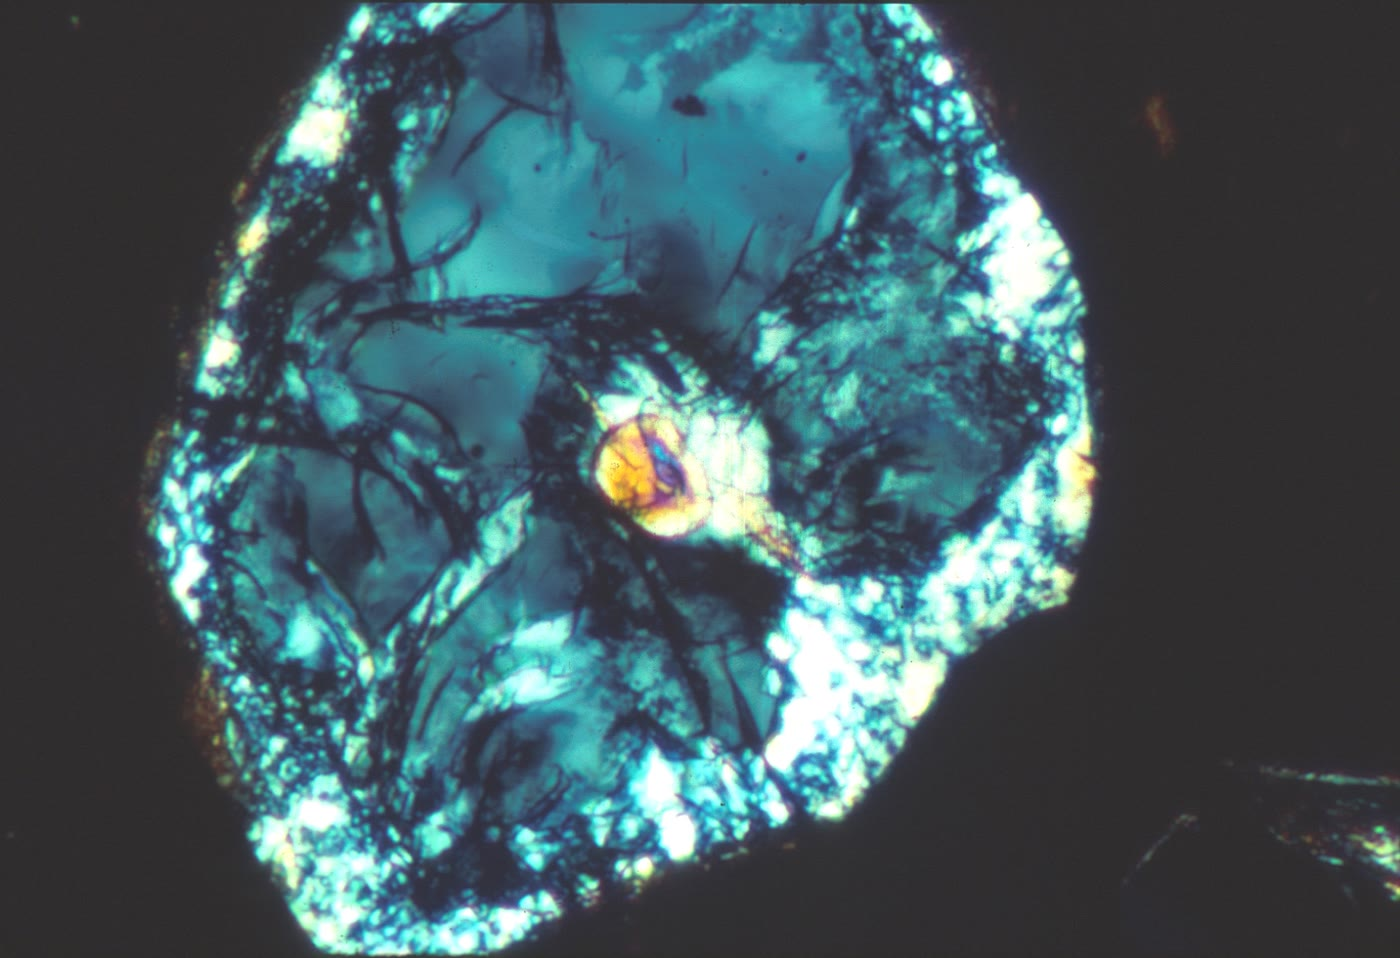
\includegraphics[width=0.62\linewidth]{images/book4/b2-11-coesite.jpg}
\par\smallskip{\small كوسيت في إكلوجيت، قطره نحو \qty{1}{mm}، في شريحة رقيقة
بين مستقطبين متعامدين: الحبّة المركزية الكبيرة كوسيت، والإطار من الحبيبات الصغيرة اللامعة
كوارتز نما منه مع انخفاض الضغط؛ والحبّة الملوّنة الصغيرة في المركز
احتواء من البيروكسين. الصورة: \mbox{\textdir TLT J.\,R. Smyth, CC BY-SA 1.0}.}
\end{omfigure}

بعد ست سنوات، وُجدت ماسات متوسط قطرها \qty{12}{\micro m} في النيس والشيست
وصخور الغارنت--البيروكسين في كتلة كوكتشيتاف في شمال كازاخستان، محتضنة في الغارنت
والزركون، اللذين حمياها من التحوّل إلى غرافيت: وقد نمت عند \qty{40}{kbar}
أو أكثر وفوق 900 إلى \qty{1000}{\celsius}. فالقشرة القارية، على خفّتها، يمكن أن
تُجرّ أكثر من مئة كيلومتر إلى الأسفل.
% ledger: ss90:diamond

أمّا كيف تعود فتخبر به ساعاتها. ففي أعمق الصخور المندسّة في الألب،
يُظهر التيتانيت المؤرَّخ في مراحل متتالية أن صخرًا كلسيًا سيليكاتيًا بلغ نحو
\qty{3.5}{GPa} عند $35.1 \pm \qty{0.9}{Ma}$، وكان عند $1 \pm \qty{0.15}{GPa}$ عند $32.9 \pm
\qty{0.9}{Ma}$، وقرب 0.4 إلى \qty{0.5}{GPa} عند $31.8 \pm \qty{0.5}{Ma}$. ومعدّلا
\omterm{def:b2:pt-paths:exhumation}{الاستخراج} المتوسطان، 3.4 ثم \qty{1.6}{cm.yr^{-1}}، يطابقان سرعات الصفائح: فقد
عادت الصخور تقريبًا بالسرعة التي نزلت بها، أسرع بكثير مما كان الحتّ يستطيع أن يكشفها
به. ويستند المؤلّفون إلى الطفوية، أي صعود القشرة الخفيفة عبر الوشاح الأكثف،
وإلى التصدّع العادي، الذي يرقّق الصخور التي فوقها.
% ledger: rh01:exhumation

\section{تحوّل قاع المحيط}\label{sec:b2:pt-paths:ocean-floor}

\begin{definition}[تحوّل قاع المحيط؛ السربنتة]\label{def:b2:pt-paths:ocean-floor}
\emph{تحوّل قاع المحيط}\index{تحوّل قاع المحيط} هو \omterm{def:b2:metamorphic-facies:metamorphism}{التحوّل الإقليمي}
لليثوسفير المحيطي قرب مراكز التباعد، بموائع مائية ساخنة
تدور تحت تدرّجات حرارية أرضية شديدة؛ وتكون إعادة التبلور غير مكتملة عمومًا
وترتفع درجة الحرارة عادةً مع العمق. و\emph{السربنتة}\index{السربنتة}
هي إماهة الصخور الغنية بالأوليفين إلى سربنتين.
\end{definition}
% ledger: scmr:types

مياه البحر المسحوبة إلى القشرة الفتية قرب محور ظهرة تسخن، وتتفاعل مع الصخور،
وتصعد من جديد. والبازلت الذي تعبره يُعاد تبلوره، على نحو غير مكتمل، إلى معادن
مائية، على مدى واسع من درجات الحرارة. وحيث يبلغ الماء \omterm{def:b2:mantle-melting:peridotites}{البيريدوتيت}، كما في
الظهرات البطيئة حيث تصعد صخور الوشاح إلى قاع البحر وتغذّي ينابيع مثل
ينابيع حقل المدينة المفقودة (مجلد السنة الأولى)، يأخذ الأوليفين الماء:
\[
\ce{2 Mg2SiO4 + 3 H2O -> Mg3Si2O5(OH)4 + Mg(OH)2},
\]
أي الفورستيريت يعطي السربنتين والبروسيت. والأحجام المولية، 43.65 للفورستيريت، و107.50
للسربنتين، و\qty{24.63}{cm^3.mol^{-1}} للبروسيت، تُظهر ما يفعله هذا بالصخر:
فتصير \qty{87.30}{cm^3} من الأوليفين \qty{132.13}{cm^3} من المواد الصلبة، أي أكثر بنسبة \qty{51}{\percent}،
وتنخفض الكثافة من 3.22 إلى \qty{2.54}{g.cm^{-3}}. فينتفخ الصخر
ويخفّ، والماء الذي ربطه ينزل معه حين تندسّ الصفيحة.
% ledger: scmr:types, rh95:serpentine, kelley:lost-city, dick:ultraslow

\begin{inthelab}[قراءة حبّة غارنت]
لقراءة مسار ضغط--حرارة، يقطع عالم الصخور أولًا شريحة رقيقة عبر مركز
حبّة غارنت، لأن مقطعًا بعيدًا عن المركز يفوّت النواة. وتحت المجهر تُرسم خريطة الاحتواءات:
حبيبات صغيرة من الكوارتز أو البيوتيت أو البلاجيوكليز أو الكيانيت انحبست أثناء نموّ
الغارنت، وقد تصطفّ أحيانًا في مسارات تحفظ تورّقًا أقدم للصخر. ثم يقيس
المسبار الإلكتروني الدقيق التركيب على امتداد خط من النواة إلى الحافة، وتُظهر خريطة
للمغنيسيوم والحديد والكالسيوم والمنغنيز نطاقات النموّ. ويُقرن كل نطاق
بالمعادن التي نمت معه: الاحتواءات للنواة، والأرضية الملامسة
للحافة. ويُطبَّق ميزان الحرارة وميزان الضغط على كل زوج، وتُؤرَّخ النطاقات حيث يسمح
معدن بذلك. ويصف \cref{ch:b2:field-lab-methods-2} الأجهزة.
\end{inthelab}

\begin{omfigure}
\centering
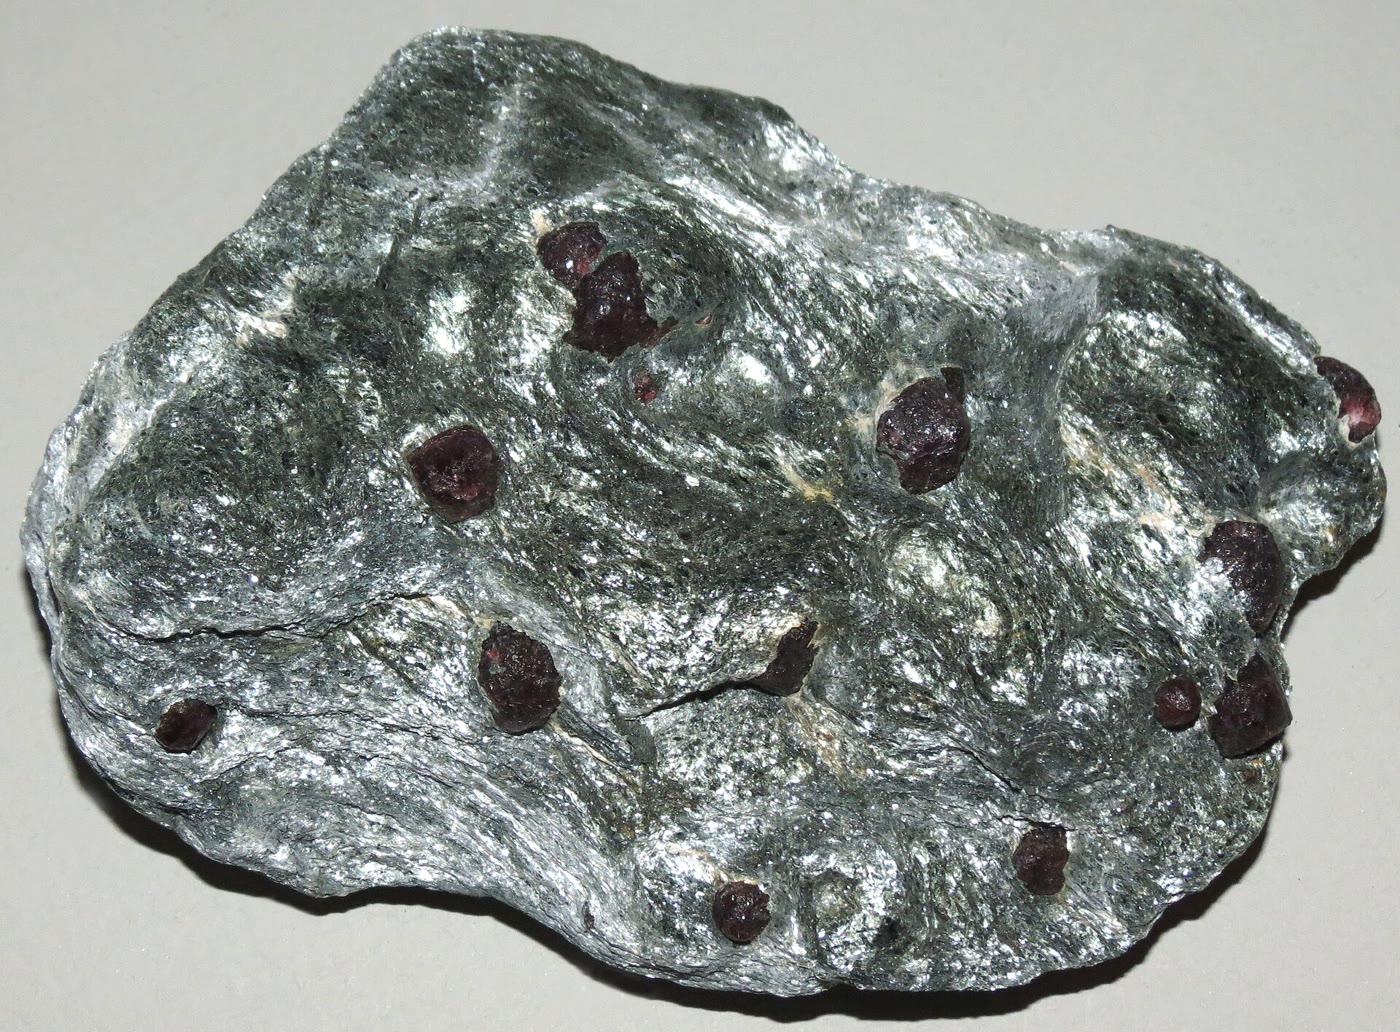
\includegraphics[width=0.62\linewidth]{images/book4/b2-11-garnet-schist.jpg}
\par\smallskip{\small شيست غارنتي: بلّورات غارنت حمراء داكنة نمت في
أرضية متورّقة من الميكا. ويمكن لكل حبّة غارنت أن تحفظ، من النواة إلى الحافة،
سجلًّا لمسار الصخر. الصورة: \mbox{\textdir TLT James St.~John, CC BY 2.0}.}
\end{omfigure}

\section{التمارين}

\begin{exercise}[$\star$]\label{exo:b2:pt-paths:1}
تحوي ست عيّنات من تكوين واحد من الحجر الطيني، جُمعت على امتداد طريق: (A) كلوريت،
مسكوفيت، كوارتز؛ (B) بيوتيت، كلوريت، مسكوفيت، كوارتز؛ (C) غارنت، بيوتيت،
مسكوفيت، كوارتز؛ (D) ستوروليت، غارنت، بيوتيت، مسكوفيت، كوارتز؛ (E) كيانيت،
ستوروليت، بيوتيت، مسكوفيت، كوارتز؛ (F) سيليمانيت، بيوتيت، مسكوفيت، كوارتز.
(أ) في أيّ نطاق من \omterm{def:b2:pt-paths:barrovian}{نطاقات بارو} تقع كلٌّ منها؟ (ب) كم خط تساوي درجة يعبر الطريق،
وما هي؟ (ج) لماذا لا تكفي معرفة خطوط تساوي الدرجة لرسم \omterm{def:b2:pt-paths:barrovian}{التدرّج التحوّلي
الحقلي}؟
\end{exercise}
% ledger: iugs:barrow

\begin{exercise}[$\star$]\label{exo:b2:pt-paths:2}
لحبّة غارنت $X_{\text{Mg}} = 0.10$ و$X_{\text{Fe}} = 0.80$، وللبيوتيت بجانبها
$X_{\text{Mg}} = 0.45$ و$X_{\text{Fe}} = 0.50$. (أ) احسب $K_D$ و$\ln K_D$.
(ب) بمعايرة هذا الفصل، احسب درجة الحرارة عند \qty{5}{kbar} وعند
\qty{7}{kbar}. (ج) هل النتيجة مقياس لدرجة الحرارة أم للضغط؟
\end{exercise}
% ledger: h97:ideal, h97:fs-reaction

\begin{exercise}[$\star$]\label{exo:b2:pt-paths:3}
يعطي ميتابيليت \qty{580}{\celsius} و\qty{6.0}{kbar}. (أ) تحت صخور كثافتها المتوسطة
\qty{2800}{kg.m^{-3}} ($g = \qty{9.81}{m.s^{-2}}$)، على أيّ عمق كان؟ (ب) أيّ
تدرّج حراري يقتضيه ذلك انطلاقًا من \qty{10}{\celsius} على السطح؟ (ج) يمرّ
خط الكيانيت $=$ السيليمانيت التجريبي بالقيمة \qty{3.67}{kbar} عند
\qty{500}{\celsius} وبالقيمة \qty{5.77}{kbar} عند \qty{600}{\celsius}: أيّ سيليكات ألومنيوم
ينبغي أن يحويها الصخر؟
\end{exercise}
% ledger: hm93:table11

\begin{exercise}[$\star$]\label{exo:b2:pt-paths:4}
\omterm{def:b2:pt-paths:ocean-floor}{لسربنتة} الفورستيريت المكتوبة في هذا الفصل: (أ) تحقّق من أن
المعادلة موزونة كتليًا، مع الكتل المولية 140.693 (فورستيريت)، و18.015 (ماء)،
و277.112 (سربنتين)، و\qty{58.320}{g.mol^{-1}} (بروسيت)؛ (ب) احسب تغيّر
حجم المواد الصلبة؛ (ج) احسب كثافتي الأوليفين والنواتج.
(د) ماذا يفعل هذا التغيّر ببيريدوتيت مسربت تحت قاع البحر؟
\end{exercise}
% ledger: rh95:serpentine

\begin{exercise}[$\star\star$]\label{exo:b2:pt-paths:5}
عايِر ميزان الحرارة من أربع من التجارب عند \qty{2.07}{kbar}: $\ln K_D =
-1.157$ و$-1.255$ عند \qty{799}{\celsius}، و$-1.738$ و$-1.826$ عند \qty{550}{\celsius}.
(أ) خذ متوسط كل زوج وجد الخط $\ln K_D = a/T + b$ المارّ بالمتوسطين.
(ب) استنتج $\Delta_r H$ و$\Delta_r S$، مع $\Delta_r V = \qty{0.311}{J.bar^{-1}}$.
(ج) قارن درجات الحرارة التي تعطيها معايرتك ومعايرة الفصل عند
\qty{5}{kbar} من أجل $K_D = 0.18$ و$0.10$ و$0.30$. ماذا تستنتج عن
استقراء معايرة؟
\end{exercise}
% ledger: h97:fs-data, h97:ideal

\begin{exercise}[$\star\star$]\label{exo:b2:pt-paths:6}
(أ) من الأحجام المولية عند \qty{298}{K} (الألماندين 115.32، والبيروب 113.12، والأنيت
154.30، والفلوغوبيت 149.65، والغروسولار 125.28، والأنورثيت 100.79، والكيانيت 44.15، والكوارتز
\qty{22.69}{cm^3.mol^{-1}})، احسب $\Delta_r V$ للتبادل ولتفاعل
GASP، وقارن بالقيمتين اللتين تستعملهما المعايرتان، \num{0.311}
و\qty{-6.21}{J.bar^{-1}}. (ب) من أجل $K_D = 0.18$، بكم كلفن يُزيح خطأ قدره
\qty{1}{kbar} درجة الحرارة؟ (ج) على امتداد خط GASP لصخر فيه
$X_{\text{Ca}}/X_{\text{an}} = 0.20$، بكم بار يُزيح خطأ قدره \qty{17}{K}
الضغط؟
\end{exercise}
% ledger: rh95:gb-gasp, rh95:al2sio5, h97:fs-reaction, kn88:gasp

\begin{exercise}[$\star\star$]\label{exo:b2:pt-paths:7}
عند \qty{600}{\celsius}، لحبّة غارنت $X_{\text{Ca}} = 0.08$ وللبلاجيوكليز بجانبها
$X_{\text{an}} = 0.30$. (أ) احسب ضغط GASP. (ب) أعد الحساب مع $X_{\text{an}} =
0.35$. (ج) على أيّ عمق كان الصخر، من أجل كثافة متوسطة قدرها \qty{2800}{kg.m^{-3}}؟
\end{exercise}
% ledger: kn88:gasp

\begin{exercise}[$\star\star$]\label{exo:b2:pt-paths:8}
استعمل أعمار التيتانيت لأعمق الصخور المندسّة في الألب: نحو \qty{3.5}{GPa} عند
$35.1 \pm \qty{0.9}{Ma}$، و\qty{1.0}{GPa} عند $32.9 \pm \qty{0.9}{Ma}$، و\qty{0.45}{GPa} عند
$31.8 \pm \qty{0.5}{Ma}$. (أ) بكثافة متوسطة قدرها \qty{3000}{kg.m^{-3}}، حوّل
الضغوط إلى أعماق. (ب) احسب معدّلي \omterm{def:b2:pt-paths:exhumation}{الاستخراج} المتوسطين وقارن بالقيمتين
المنشورتين 3.4 و\qty{1.6}{cm.yr^{-1}}. (ج) ما عدم اليقين في المجال الزمني
الأول، وأيّ مدى من المعدّلات يسمح به؟ (د) قارن بمعدّل الحتّ في
نموذج الإثخان، \qty{0.5}{mm.yr^{-1}}.
\end{exercise}
% ledger: rh01:exhumation

\begin{exercise}[$\star\star$]\label{exo:b2:pt-paths:9}
من أجل $K_D = 0.18$ عند \qty{5}{kbar}، (أ) احسب $\partial T/\partial\ln K_D$
و$\partial T/\partial P$ من القضية؛ (ب) مع $\sigma_{\ln K_D} = 0.05$ (خطأ
قدره \qty{5}{\percent} على $K_D$) و$\sigma_P = \qty{1}{kbar}$، احسب $\sigma_T$.
(ج) أيّ الخطأين هو الغالب؟ قارن بعدم اليقين البالغ \qty{25}{\celsius} الذي تدّعيه
أفضل المعايرات.
\end{exercise}
% ledger: h97:ideal

\begin{exercise}[$\star\star\star$]\label{exo:b2:pt-paths:10}
لحافة حبّة غارنت $X_{\text{Mg}} = 0.10$، $X_{\text{Fe}} = 0.75$، $X_{\text{Ca}} = 0.07$؛
ولبيوتيت الأرضية $X_{\text{Mg}} = 0.42$، $X_{\text{Fe}} = 0.52$؛ وللبلاجيوكليز
$X_{\text{an}} = 0.25$. (أ) طبّق طريقة هذا الفصل، بدءًا من \qty{6}{kbar}،
حتى تتغيّر درجة الحرارة بأقل من \qty{1}{K}. (ب) أيّ سيليكات ألومنيوم ينبغي أن
يحويها الصخر (استعمل الخط التجريبي في \cref{exo:b2:pt-paths:3})؟ (ج) لماذا يجب أن يستعمل ميزان الضغط
سيليكات الألومنيوم الحاضرة فعلًا؟
\end{exercise}
% ledger: h97:ideal, kn88:gasp, hm93:table11

\begin{exercise}[$\star\star\star$]\label{exo:b2:pt-paths:11}
مع $\kappa = \qty{1e-6}{m^2.s^{-1}}$: (أ) احسب زمن الاسترخاء في
القضية من أجل $L = \qty{35}{km}$ ومن أجل $L = \qty{70}{km}$. (ب) يحتّ النموذج
\qty{35}{km} في 70 مليون سنة؛ قارن هذا الزمن بزمني (أ). (ج) اشرح،
من هذه الأزمنة، لماذا يبلغ صخر النموذج ذروته الحرارية بعد ذروته
الضغطية. (د) لو كان الحتّ أسرع بعشر مرات، فما الذي سيتغيّر في المسار؟
\end{exercise}
% ledger: delaney:conductivity, et84:ptt

\begin{exercise}[$\star\star\star$]\label{exo:b2:pt-paths:12}
خذ قشرة سمكها \qty{35}{km} وكثافتها \qty{2800}{kg.m^{-3}} فوق وشاح كثافته
\qty{3300}{kg.m^{-3}}. (أ) على أيّ عمق يبلغ الضغط \qty{28}{kbar}، وهو
الحدّ الأدنى لكوسيت دورا مايرا؟ (ب) وعلى أيّ عمق يبلغ \qty{40}{kbar}، لماسات كوكتشيتاف؟
(ج) أيّ تدرّج متوسط تقتضيه \qty{700}{\celsius} على عمق (أ)، وفي أيّ
متتالية يقع؟ (د) بسرعة \qty{3.4}{cm.yr^{-1}}، كم يستغرق الصعود من عمق
(أ) إلى \qty{35}{km}؟
\end{exercise}
% ledger: chopin84:coesite, ss90:diamond, rh01:exhumation

\section{مسألة: رحلة حبّة غارنت}

\begin{problem}[{مسألة نهاية الأسبوع --- القياس الحراري الضغطي، والمسار ومعدّل الاستخراج لشيست
واحد}]
\label{pb:b2:pt-paths:1}
يحوي شيست كيانيتي--غارنتي--بيوتيتي حبّات غارنت لها نواة وحافة. وتحتضن النواة
بيوتيتًا وبلاجيوكليزًا وكيانيتًا؛ وتلامس الحافة بيوتيت الأرضية وبلاجيوكليزها.
وحول حبّات الغارنت حلّ السيليمانيت محلّ بعض الكيانيت، وعند حوافّ
حبّات الغارنت نما بعض الكلوريت. والتحاليل هي:
\begin{center}
\small
\begin{tabular}{@{}lccc@{}}
\hline
 & $X_{\text{Mg}}$ & $X_{\text{Fe}}$ & $X_{\text{Ca}}$ أو $X_{\text{an}}$\\
\hline
نواة الغارنت & 0.080 & 0.760 & 0.050\\
بيوتيت محتبس في النواة & 0.40 & 0.58 & ---\\
بلاجيوكليز محتبس في النواة & --- & --- & 0.25\\
حافة الغارنت & 0.120 & 0.720 & 0.060\\
بيوتيت الأرضية & 0.46 & 0.53 & ---\\
بلاجيوكليز الأرضية & --- & --- & 0.28\\
\hline
\end{tabular}
\end{center}
استعمل ميزان الحرارة غارنت--بيوتيت وميزان الضغط GASP في هذا الفصل (خلط مثالي)،
و$R = \qty{8.314}{J.mol^{-1}.K^{-1}}$، و$g = \qty{9.81}{m.s^{-2}}$، وكثافة متوسطة قدرها
\qty{2800}{kg.m^{-3}} فوق الصخر، وقرّب كل نسبة إلى أربعة أرقام عشرية.

\noindent\textbf{الجزء الأول --- درجات الحرارة.}
\begin{enumerate}
\item احسب $X_{\text{Mg}}/X_{\text{Fe}}$ في نواة الغارنت وفي البيوتيت
المحتبس، ثم $K_D$ و$\ln K_D$ للنواة.
\item افعل الشيء نفسه للحافة وبيوتيت الأرضية.
\item احسب درجة حرارة النواة عند \qty{6}{kbar}.
\item احسب درجة حرارة الحافة عند \qty{6}{kbar}.
\item بكم كلفن يغيّر خطأ قدره \qty{1}{kbar} درجتي الحرارة هاتين؟
\item لماذا تُقرن النواة بالبيوتيت المحتبس، والحافة ببيوتيت
الأرضية؟
\end{enumerate}

\noindent\textbf{الجزء الثاني --- الضغوط.}
\begin{enumerate}[resume]
\item احسب ضغط الأعضاء الطرفية $P_0$ لتفاعل GASP عند درجتي الحرارة
في السؤالين~3 و~4.
\item احسب ضغط GASP للنواة عند درجة حرارة السؤال~3.
\item احسب ضغط GASP للحافة عند درجة حرارة السؤال~4.
\item أعد حساب درجة حرارة الحافة عند ضغط السؤال~9، ثم ضغطها
عند درجة الحرارة هذه، ثم درجة الحرارة مرة أخرى. أعطِ درجة حرارة الحافة
وضغطها.
\item افعل الشيء نفسه مرة واحدة للنواة. لماذا تتغيّر قليلًا جدًّا؟
\item حوّل ضغطي النواة والحافة إلى أعماق.
\item يمرّ خط الكيانيت $=$ السيليمانيت التجريبي بالقيم 3.67 و5.77
و\qty{7.86}{kbar} عند 500 و600 و\qty{700}{\celsius}. أيّ سيليكات ألومنيوم كانت مستقرة
حين نمت النواة، وحين نمت الحافة؟ وهل كيانيت النواة متّسق؟
\end{enumerate}

\noindent\textbf{الجزء الثالث --- المسار.}
\begin{enumerate}[resume]
\item بين النواة والحافة، بكم تغيّرت درجة الحرارة والضغط؟
وهل كانت حبّة الغارنت تنمو على \omterm{def:b2:pt-paths:paths}{المسار التقدّمي} أم التراجعي؟
\item يحلّ السيليمانيت محلّ الكيانيت حول حبّات الغارنت. عند درجة حرارة الحافة،
تحت أيّ ضغط يجب أن يكون الصخر قد مرّ ليحدث ذلك؟ وماذا فعل الصخر
بعد أن نمت الحافة؟
\item ينمو الكلوريت عند حوافّ حبّات الغارنت. أيّ جزء من المسار يسجّل؟
\item ارسم المسار: النواة، الحافة، السيليمانيت، الكلوريت. هل هو باتجاه عقارب الساعة أم بعكسها؟
وأيّ ذروة جاءت أولًا؟
\item يوصل نموذج الإثخان في هذا الفصل صخره إلى ذروة حرارية قدرها
\qty{593}{\celsius} عند \qty{7.8}{kbar}. هل مسار الشيست من النوع نفسه؟
\end{enumerate}

\noindent\textbf{الجزء الرابع --- بأيّ سرعة.}
\begin{enumerate}[resume]
\item تعطي حافة الغارنت عمرًا بطريقة الساماريوم--النيوديميوم قدره $412.0 \pm \qty{1.5}{Ma}$، يؤخذ
عمرًا للذروة؛ ويعطي مسكوفيت الأرضية عمرًا بالأرغون قدره $398.0 \pm
\qty{1.0}{Ma}$، وهو الزمن الذي برد فيه الصخر عبر \qty{405}{\celsius}. احسب
معدّل التبريد المتوسط بينهما.
\item تفترض درجة حرارة الانغلاق \qty{405}{\celsius} تبريدًا بمعدل
\qty{10}{\celsius} لكل مليون سنة. هل يستدعي معدّل السؤال~19 قيمة أعلى أم
أدنى، ولماذا؟
\item عند \qty{398}{Ma}، خذ تدرّجًا حراريًا أرضيًا قدره \qty{30}{\celsius\per\km} انطلاقًا من
\qty{10}{\celsius} على السطح. على أيّ عمق انغلق المسكوفيت؟
\item كم صعد الصخر بين الذروة وانغلاق المسكوفيت؟
\item ما عدم اليقين في المجال الزمني؟
\item احسب \omterm{def:b2:pt-paths:exhumation}{معدّل الاستخراج} المتوسط من الذروة إلى انغلاق المسكوفيت، بالمليمترات
في السنة ومقرّبًا إلى العُشر: الرقم الأساسي في هذه المسألة.
\end{enumerate}
\end{problem}
% ledger: h97:ideal, h97:fs-reaction, kn88:gasp, hm93:table11, h09:muscovite, scmr:ptt, et84:ptt
